% % % % % % % %  MDT UFSM 2021  % % % % % % % % 
%% Arquivo base para o documento - ver. 1.0 %%
% % % % % % % % % % % % % % % % % % % % % % % % 


% % % OPCOES DE COMPILACAO
% % % PAGINACAO
% % % PAGINACAO SIMPLES (FRENTE): PARA TRABALHOS COM MENOS DE 100 PAGINAS
\documentclass[oneside,openright,12pt]{ufsm_2021} %%%%% OPCAO PADRAO -> PAGINACAO SIMPLES. PARA TRABALHOS COM MAIS DE 100 PAGINAS COMENTE ESTA LINHA E DESCOMENTE A LINHA 
% % % % % % % % % % % % % % % % % % % % % % % % % % % % % % % % % % % % % % %
% PAGINACAO DUPLA (FRENTE E VERSO): PARA TRABALHOS COM MAIS DE 100 PAGINAS
% \documentclass[twoside,openright,12pt]{ufsm_2021}  %%%% PARA TRABALHOS COM MAIS DE 100 PAGINAS DESCOMENTE AQUI
% % % % % % % % % % % % % % % % % % % % % % % % % % % % % % % % % % % % %




% % % %  CODIFICACAO DO TEXTO 
% % % %  POR PADRAO USA-SE UTF8. PARA APLICAR A CODIFICACAO OESTE EUROPEU (ISO 8859-1) DESCOMENTE A LINHA ABAIXO. ELA ATIVA A OPCAO "latin1" DO PACOTE "inputenc"
%% \oesteeuropeu
% % % % % % % % % % % 



% % % % % % % % PACOTES PESSOAIS % % % % % % % %  
\usepackage{lipsum}
\usepackage{quoting}
\usepackage[utf8]{inputenc}
\usepackage[T1]{fontenc}
\usepackage[brazil]{babel}
\usepackage{hyperref}
\usepackage{amsmath}
% \usepackage{aas_macros}
% \usepackage{natbib}
% \usepackage[sorting=none]{biblatex}
% \usepackage[numbers]{natbib}
% \usepackage{aastex_hack}
% % % % % % % % DEFINICOES PESSOAIS % % % % % % % %







% % % % % % % % % % % % % % % % % % % % % % % % % % % % % % % % % % % % % % % % % % % 




% % % % % % % % % % % % % % % % % % % % % % % % % % % % % % % % % 
% % % % % % % % % % % % DADOS DO TRABALHO % % % % % % % % % % % % 
% % % % % % % % % % % % % % % % % % % % % % % % % % % % % % % % % 

% % % % % % % % % % INFORMACOES INSTITUCIONAIS % % % % % % % % % % 


% % CENTRO DE ENSINO DA UFSM
\centroensino{Centro de Tecnologia}  %%% NOME POR EXTENSO
\centroensinosigla{CT}  %%% SIGLA

% % CURSO DA UFSM
\nivelensino{Pós-Graduação}  %%%%%%% NIVEL DE ENSINO 
\curso{Engenharia Elétrica}   %%%%% NOME POR EXTENSO
\ppg{PPGEE}   %%%%%% SIGLA
\statuscurso{Programa}  %%%% STATUS= {Programa} ou {Curso}
% \EAD  %%%% para cursos EAD
% % % %  LOCAL DO CAMPUS OU POLO
\cidade{Santa Maria}
\estado{RS}


% % % % % % % % % % INFORMACOES DO AUTOR % % % % % % % % % % 
\author{Leonardo Felipe da Silva dos Santos}   %%%%% AUTOR DO TRABALHO
\sexo{M} %%%% SEXO DO AUTOR -> M=masculino   F=feminino (IMPORTANTE PARA AJUSTAR PAGINAS PRE-TEXTUAIS)
\grauensino{Doutorado}    %%%%%%%% GRAU DE ENSINO A SER CONCLUIDO
\grauobtido{Doutor}    %%%%% TITULO OBTIDO
\email{leonardo.santos@acad.ufsm.br}   %%%% E-MAIL PARA CATALOGRAFICA (COPYRIGHT) - OBRIGATORIO
\endereco{Rua João Atillio Zampieri, n. 709, apto 201} %%%% TELEFONE PARA CATALOGRAFICA (COPYRIGHT) (CAMPO OPICIONAL -- CASO NAO POSSUA OU NAO QUEIRA DIVULGAR COMENTE A LINHA)
\fone{55 99992 1300}   %%%% TELEFONE PARA CATALOGRAFICA (COPYRIGHT) FORMATO {11 2222 3333} (CAMPO OPICIONAL -- CASO NAO POSSUA OU NAO QUEIRA DIVULGAR COMENTE A LINHA)
% \fax{11 2222 3333}   %%%% FAX PARA CATALOGRAFICA (COPYRIGHT) FORMATO {11 2222 3333} (CAMPO OPICIONAL -- CASO NAO POSSUA OU NAO QUEIRA DIVULGAR COMENTE A LINHA)


% % % % % % % % % % INFORMACOES DA BANCA % % % % % % % % % % 
% OBSERVACOES: O CAMPO ORIENTADOR EH OBRIGATORIO E NAO DEVE SER COMENTADO
% % % % % %    OS DEMAIS MEMBROS DA BANCA (COOREIENTADOR E DEMAIS PROFESSORES) QUANDO COMENTADOS NAO APARECEM NA FOLHA DE APROVACAO (O LAYOUT DA FOLHA DE APROVACAO ESTA PREPARADO PARA O ORIENTADOR E ATE MAIS 4 MEMBROS NA BANCA
\orientador{João da Silva}{Dr}{AAAA}{M}{P}  %%%INFORMACOES SOBRE ORIENTADOR: OS CAMPOS SAO:{NOME}{SIGLA DA TITULACAO}{SIGLA DA INSTITUICAO DE ORIGEM}{SEXO} M=masculino   F=feminino {PARTE DA BANCA?} P=presidente  M=Membro  N=Nao faz parte
\coorientador{Maria da Costa}{Dra}{AAAA}{F}{M} %%%INFORMACOES SOBRE CO-ORIENTADOR: OS CAMPOS SAO:{NOME}{SIGLA DA TITULACAO}{SIGLA DA INSTITUICAO DE ORIGEM}{SEXO} M=masculino   F=feminino {PARTE DA BANCA?} P=presidente  M=Membro  N=Nao faz parte
\bancaum{Banca Um}{Dr}{AAAA}{F}{M}  %%%INFORMACOES SOBRE PRIMEIRO NOME DA BANCA: OS CAMPOS SAO:{NOME}{SIGLA DA TITULACAO}{SIGLA DA INSTITUICAO DE ORIGEM}{SEXO} M=masculino   F=feminino {PARTE DA BANCA?} P=presidente  M=Membro  N=Nao faz parte
%\bancadois{Banca Dois}{Dr}{BBBB}  %%%INFORMACOES SOBRE SEGUNDO NOME DA BANCA: OS CAMPOS SAO:{NOME}{SIGLA DA TITULACAO}{SIGLA DA INSTITUICAO DE ORIGEM}
% \bancatres{Banca Três}{Dra}{CCCC} %%%INFORMACOES SOBRE TERCEIRO NOME DA BANCA: OS CAMPOS SAO:{NOME}{SIGLA DA TITULACAO}{SIGLA DA INSTITUICAO DE ORIGEM}
% \bancaquatro{Banca Quatro}{Dr}{DDDD} %%%INFORMACOES SOBRE QUARTO NOME DA BANCA: OS CAMPOS SAO:{NOME}{SIGLA DA TITULACAO}{SIGLA DA INSTITUICAO DE ORIGEM}
% \bancacinco{Banca Cinco}{Dra}{EEEE} %%%INFORMACOES SOBRE QUARTO NOME DA BANCA: OS CAMPOS SAO:{NOME}{SIGLA DA TITULACAO}{SIGLA DA INSTITUICAO DE ORIGEM}
% \supervisor{Al Paccino}{Dr}{MAFIA}{M}{N} %%%INFORMACOES SOBRE SUPERVISOR (indicado para estagios): OS CAMPOS SAO:{NOME}{SIGLA DA TITULACAO}{SIGLA DA INSTITUICAO DE ORIGEM}{SEXO} M=masculino   F=feminino {PARTE DA BANCA?} P=Presidente  M=Membro  N=Nao faz parte



% % % % % % % % % % REALIZACAO POR VIDEO CONFERENCIA (MEMORANDO 04/2016 BIBLIOTECA CENTRAL UFSM)
% \videoconferencia % % % % QUANDO O ACADEMICO DEFENDE POR VIDEO CONFERENCIA (PERMITIDO PELO ARTIGO 82 DO REGIMENTO GERAL DA PRPGP/UFSM). PARA DEFESAS NAS QUAIS O ACADEMICO ESTA PRESENTE COMENTE ESTA LINHA
% % % % QUANDO UM DOS MEMBROS DA BANCA PARTICIPA POR VIDEO CONFERENCIA INDICAR O MEMBRO DE ACORDO COM A LISTA ABAIXO. CASO CONTRARIO MANTER A PALAVRA "NAO". SAO PERMITIDOS, PELO REGIMENTO PRGPGP (ARTIGO 83) ATE 2 MEMBROS 
\videoconferenciabancap{NAO}  %%%% PRIMEIRO MEMBRO
\videoconferenciabancas{NAO}  %%%%% SEGUNDO MEMBRO
% % O > ORIENTADOR
% % CO > COORIENTADOR% % % % QUANDO UM DOS MEMBROS DA BANCA PARTICIPA POR VIDEO CONFERENCIA INDICAR O MEMBRO DE ACORDO COM A LISTA ABAIXO. CASO CONTRARIO MANTER A PALAVRA "NAO". SAO PERMITIDOS, PELO REGIMENTO PRGPGP ATE 2 MEMBROS.
% % 1 > BANCA UM
% % 2 > BANCA DOIS
% % 3 > BANCA TRÊS
% % 4 > BANCA QUATRO
% % 5 > BANCA CINCO
% % S > SUPERVISOR
% % % % % % % % % % % % % % % % % % % % % % % % % % % % % % % % % % % % 



% % % % % % % % % % INFORMACOES SOBRE O TRABALHO % % % % % % % % % %
% % % %  TITULO E SUBTITULO DO TRABALHO: ELES NÃO DEVEM ULTRAPASSAR, JUNTOS, 3 LINHAS NA COMPILAÇÃO DA CAPA. 
% SE O TRABALHO POSSUI SUBTITULO, ADICIONE ':' DENTRO DAS CHAVES ABAIXO 
\titulo{Eu ainda Não sei} %% NAO EH NECESSARIO CAPITALIZAR
% % % %  TITULO DO TRABALHO EM INGLES
% SE O TRABALHO POSSUI SUBTÍTULO, ADICIONE ':' DENTRO DAS CHAVES ABAIXO 
\englishtitle{I dont know}  %% NAO EH NECESSARIO CAPITALIZAR


% % % % O SUBTÍTULO É OPCIONAL, SE NÃO FOR USADO AS LINHAS ABAIXO DEVEM SER COMENTADAS

% SE O TRABALHO POSSUI SUBTÍTULO, ADICIONE ':' DENTRO DAS CHAVES ABAIXO 
\subtitulo{Preciso colocar?} %% NAO EH NECESSARIO CAPITALIZAR
% % % %  SUB TITULO DO TRABALHO EM INGLES
\subenglishtitle{Need this?}  %% NAO EH NECESSARIO CAPITALIZAR

% % % AREA DE CONCENTRACAO DO TRABALHO (CNPQ)
\areaconcentracao{Sistemas de Energia}
% % % TIPO DE TRABALHO - MANTER APENAS UMA LINHA DESCOMENTADA
\tese  %% Tese de <nivel de ensino>
% \qualificacao %% Exame de Qualificação de <nivel de ensino>
% \dissertacao %% Dissertacao de <nivel de ensino>
% \monografia %% Monografia
% \monografiag  %% Monografia (nao exibe area de concentracao)
% \tf  %% Trabalho Final de <nivel de ensino>
% \tfg  %% Trabalho Final de Graduacao (nao exibe area de concentracao)
% \tcc  %% Trabalho de Conclusao de Curso
% \tccg  %% Trabalho de Conclusao de Curso (nao exibe area de concentracao)
% \relatorio  %% Relatório de Estágio (nao exibe area de concentracao)
% \generico   %%% Alternativa para aqueles cursos que nao recebem o titulo de bacharel ou licenciado. Ex: engenharia, arquitetura, etc... Os campos abaixo tambem devem ser preenchidos
%     \tipogenerico{Tipo de trabalho em português}
%     \tipogenericoen{Tipo de trabalho em inglês}
%     \concordagenerico{o}
%     \graugenerico{Engenheiro Eletricista}
% % % DATA DA DEFESA 
\data{25}{09}{2025} %% FORMATO {DD}{MM}{AAAA}



% % % % %  ALGUMAS ENTRADAS PRE-TEXTUAIS
% % % % CASO NAO QUEIRA UTILIZA-LAS COMENTE A LINHA DE COMANDO
% % % EPIGRAFE
\epigrafe{Um grama de ação vale uma tonelada de teoria.}{ENGELS, Friedrich} %ESTRUTURA DE CAMPOS -> {Texto}{Autor}
% % % DEDICATORIA
\dedicatoria{Ao fim dos tempos}
% % % %  AGRADECIMENTOS
\agradecimentos{A mim!}

% % % % %  RESUMO E PALAVRAS CHAVE DO RESUMO - OBRIGATORIO PARA MDT-UFSM
\resumo{
Escreva seu resumo aqui! Você pode digitá-lo diretamente neste arquivo ou usar o comando input. O resumo deve ter apenas uma página, desde o cabeçalho até as palavras chave. Caso seu resumo seja maior, use comandos para diminuir espaçamento e fonte (até um mínimo de 10pt) no texto.  Segundo a MDT, é preciso que os resumos tenham, no máximo, 250 palavras para trabalhos de conclusão de curso de graduação, pós-graduação e iniciação científica e até 500 palavras para dissertações e teses.
}
\palavrachave{Palavra Chave 1. Palavra 2. Palavra 3. (...)}
% "... deverão constar, no mínimo, três palavras-chave, iniciadas em
% letras maiúsculas, cada termo separado dos demais por ponto, e
% finalizadas também por ponto." MDT 2012

% % % % %  ABSTRACT E PALAVRAS CHAVE DO RESUMO - OBRIGATORIO PARA MDT-UFSM
\abstract{
Write your abstract here! As recomendações do resumo também se aplicam ao abstract. \lipsum[0-1]
}
\keywords{Keyword 1. Keyword 2. Keyword 3. (...)}


% % %  ATIVACAO DE LISTAS E PAGINAS ESPECIAIS
% % %  PARA QUE APARECAO NAO NO TEXTO DESCOMENTE A LINHA ABAIXO -> POR PADRAO TODAS ESTAO ATIVIDADAS

% % LISTA DE FIGURAS 
% \semfiguras   %%(QUANDO ATIVIDA NAO EXIBE A LISTA)
% % LISTA DE GRAFICOS 
% \semgraficos   %%(QUANDO ATIVIDA NAO EXIBE A LISTA)
% % LISTA DE ILUSTRACOES 
% \semilustracoes  %%(QUANDO ATIVIDA NAO EXIBE A LISTA)
% % LISTA DE TABELAS 
% \semtabelas   %%(QUANDO ATIVIDA NAO EXIBE A LISTA)
% % LISTA DE QUADROS 
% \semquadros   %%(QUANDO ATIVIDA NAO EXIBE A LISTA)
% % LISTA DE APENDICES 
% \semapendices  %%(QUANDO ATIVIDA NAO EXIBE A LISTA)
% LISTA DE ANEXOS 
% \semanexos   %%(QUANDO ATIVIDA NAO EXIBE A LISTA)


% % % %  LISTA DE ABREVIATURAS - AMBIENTE TABULAR
%%%%%%%% para não utilizar comente as linhas abaixo.
\abreviaturamax{SIGLAMAX} %%%% coloque aqui a maior sigla (indentacao)
\listadeabreviaturas{
	SIGLA1 & Nome Completo da Sigla 1 \\
	SIGLA2 & Nome Completo da Sigla 2 \\
	SIGLAMAX &	Nome Completo da Sigla MAX \\
}


% % % %  LISTA DE SIGLAS - AMBIENTE TABULAR
%%%%%%%% para não utilizar comente as linhas abaixo.
\siglamax{SIGLAMAX} %%%% coloque aqui a maior sigla (indentacao)
\listadesiglas{
SIGLA1 & Nome Completo da Sigla 1 \\
SIGLA2 & Nome Completo da Sigla 2 \\
SIGLAMAX &	Nome Completo da Sigla MAX \\
}


% % % %  LISTA DE SIMBOLOS
%%%%%%%% OBS: O espaco entre colchetes \item[] e um ambiente matematico
%%%%%%%% para não utilizar comente as linhas abaixo.
\simbolomax{(Re)2} %%%% coloque aqui o maior simbolo (indentacao)
\listadesimbolos{
\item[u_*]	Escala de velocidade de fricção	
\item[w_*]	Escala de velocidade convectiva
\item[(Re)^2]	Maior simbolo da lista
}


% % % FICHA CATALOGRAFICA
\semcatalografica  %%%%  (QUANDO ATIVIDA NAO EXIBE A FICHA CATALOGRAFICA NECESSITA DO ARQUIVO DA FICHA: ficha_catalografica.pdf
% % % A FICHA CATALOGRAFICA FORNECIDA PELA UFSM EH UM PDF DO TAMANHO A4
% % % EH POSSIVEL GERA-LA NO SITE http://cascavel.ufsm.br/ficha_catalografica/
% % % OS COMANDOS ABAIXO DEFINEM AS MARGENS PARA CORTAR A FICHA FORNECIDA E COLOCA-LA COMO UMA FIGURA NO DOCUMENTO LATEX
\margemesquerda{1.9}   %%%% CORTE DE MARGEM ESQUERDA EM CM
\margemdireita{1.5}   %%%% CORTE DE MARGEM DIREITA EM CM
\margemsuperior{2.75}  %%%% CORTE DE MARGEM SUPERIOR EM CM
\margeminferior{2.9} %%%% CORTE DE MARGEM INFERIOR EM CM
% % %  DICA: IMPRIMA UMA COPIA DA FICHA CATALOGRAFICA E FACA A MEDIDA DAS MARGENS!





% % FOLHA DE ERRATA (versao rudimentar...pode ser aprimorado)
% % para não utilizar comente as linhas abaixo.
% % deve ser preenchida como um ambiente tabular de quatro colunas:
% % pagina & linha & onde se le & leia-a se \\
% \errata{}
% % % % % % % % % % % % % % % % % % % % % % % % % % % % % % % % % % % % % % % % % % % % % % 


% % % % % % % % % % % % % % % % % % % % % % % % % % % % % % % % % % % % % % 
% % % % % % % % % % % %  OPCOES DE FORMATACAO % % % % % % % % % % % % % % %
% % % % % % % % % % % % % % % % % % % % % % % % % % % % % % % % % % % % % % 
% % % CAPITULO: por padrao alinhado a esquerda. Para ativar alinhamento centralizado descomente o comando abaixo

% \centralizado  %%%% <<< centraliza todos os capitulos

% % % % % % % % % % % % % % % % % % % % % % % % % % % % % % % % % % % % % %
% % % FONTES: descomente uma das opcoes. caso nenhuma seja ativada a clase usara a fonte padrao do latex

%% helvetica
\usepackage[scaled]{helvet}
% \usepackage[abbr,dcucite]{harvard}
\renewcommand*\familydefault{\sfdefault}

%% arial
% \renewcommand{\rmdefault}{phv} % Arial
% \renewcommand{\sfdefault}{phv} % Arial

%%times
% \usepackage{mathptmx}

% % % % % % % % % % % % % % % % % % % % % % % % % % % % % % % % % % % % % % 
% % % % % % % % % % % % % % % % % % % % % % % % % % % % % % % % % % % % % % 
% % % % % % % % % % % % % % % % % % % % % % % % % % % % % % % % % % % % % % 
% % % % % % % % % % % % % % % % % % % % % % % % % % % % % % % % % % % % % % 


% % % % % % % % % % % % % % % % % % % % % % % % % % % % % % % % % % % % % % 
% % % % % % % % % % % % % % % % % % % % % % % % % % % % % % % % % % % % % % 
% % % % % % % % % % % %  INICIO DO DOCUMENTO  % % % % % % % % % % % % % % %
% % % % % % % % % % % % % % % % % % % % % % % % % % % % % % % % % % % % % % 
% % % % % % % % % % % % % % % % % % % % % % % % % % % % % % % % % % % % % %


\begin{document}



% % % % % % % % % % % % % % % % % % % % % % % % % % % % % % % % % % % % % % 
\pretextual  %%%% GERA AS PAGINAS PRE-TEXTUAIS   
% % % % % % % % % % % % % % % % % % % % % % % % % % % % % % % % % % % % % % 

% % % % % % % % % % % % % % % % % % % % % % % % % % % % % % % % % % % % % % 
% % % % % CORPO DO TRABALHO - INCLUA OS SEUS TEXTOS AQUI
% % % % % SUGESTAO -> UTILIZE ARQUIVOS EXTERNOS A PARTIR DO COMANDO \input
% % % % % % % % % % % % % % % % % % % % % % % % % % % % % % % % % % % % % % 
% % % % % % % % % % INICIO DAS PAGINAS TEXTUAIS % % % % % % % % % % % % % % 
% % % % % % % % % % % % % % % % % % % % % % % % % % % % % % % % % % % % % % 

\chapter{Introdução}
\section{Considerações Gerais}

\par A necessidade da energia elétrica permeia os aconteceimentos do cotidiano humano. Desde o despertar até a hora que dormimos necessitamos de energia elétrica. A viabilidade do alcance da energia elétrica se faz necessárias para todos quais os setores da sociedade. A energia elétrica é o principal fator para crescimento demográfico e também de capital da socidade. Segudo o Programa Nacional de Amostras de Domicílios (PNAD) em 2022, cerca de 12,6\% da população brasileira se encontra nas areas rurais, um decaimento de 2,68\% em relação a 2015.

\par Isso pode ser um acaso da baixa cobertura de serviços públicos, falta de investimento em infraestutura, segundo o PNAD cerca de 16,12\% da população total do brasil, não tem acesso a rede de água. Grande parte dos quais não tem acesso a rede de abastecimento de água se encontra nas regiões rurais do Brasil. Segundo a \cite{epe_balanco_2024} o consumo de energia pelas zonas rurais é apenas de 6,5\% do total de energia elétrica consumida no Brasil. Isso pode ser um indicativo de que a energia elétrica não é um fator preponderante para o crescimento demográfico e econômico da população rural.

\par Desde 1980 o Brasil, vive iniciativas públicas e privadas, para implemento da energia elétrica em zonas rurais, com o intuito de promover o desenvolvimento econômico destas áreas. Dentre todas as iniciativas podemos citar, programas como Clic Rural I e II (1984/1989 e 1990); Interluz (1989/1991); PROLUZ I e II (1990/1992 e 1995/1999); PRODEEM (1994). Luz da Terra (1996/2002); Luz no Campo (1999/2003) e Luz para Todos (2003/2025).
\par Todos estes programas visam a universalização do acesso a energia elétrica, com o intuito de promover o desenvolvimento econômico e social das áreas rurais. Assim como também promover a inclusão social e a redução da pobreza. O programa Luz para Todos, é o maior programa de eletrificação rural do mundo, com mais de 15 milhões de pessoas atendidas, e mais de 4 milhões de ligações elétricas realizadas. 

\par O programa Luz Para Todos, do Ministério de Minas e Energia (MME), é o  programa de universalização de Energia Elétrica, tem como objetivo atender 100\% da população brasileira, tanto em zonas rurais como em cidades. A universalização da energia elétrica no Brasil, Lei N°10.438/2002, define que os serviços energia elétrica, públicos e privados, devem investir na eletrificação total do Brasil de forma gratuíta e universal. Sem ônus aos solicitantes, desde que se atenda aos requisitos listados pela Agência Nacional de Energia Elétrica (ANEEL), sendo eles:

\pagebreak

\begin{itemize}
	\item Enquadramento no Grupo B;
	\item Carga instalada na unidade consumidora de até 50kW;
	\item Possa ser efetivada em tensão inferior a 2,3kV, ainda que necessário a extensão da rede primária de tensão igual ou inferior a 138kV, ou se necessário atendida por sistemas isolados;
	\item Por fim não existta unidade consumidora com fornecimento de energia elétrica na mesma propriedade.
\end{itemize}

\par Para unidades consumidoras individuais situadas em comunidades indígenas e quilombolas, a conexão elétrica pode ser gratuita, desde que satisfeitas as condições estipuladas pelas normativas nº 950 e 1000 \cite{aneel_resolucao_2021}\cite{aneel_resolucao_2022}. A viabilidade econômica da expansão da rede para essas localidades é comprometida pela distância e pelo consumo reduzido. Caso o consumidor precise elevar sua capacidade de carga, seja pela adoção de novas tecnologias agrícolas, pecuárias ou outras, será necessária uma contrapartida financeira à distribuidora. Tal elevação da demanda geralmente implica a utilização de motores trifásicos, notórios por sua maior eficiência em relação aos monofásicos. Existem alternativas para contornar o elevado investimento exigido pelos sistemas de distribuição trifásicos \cite{fandi_sistema_2013}.

\par As maiores iniciativas da composição dos programas eram voltadas para a expansão da rede elétrica, com redes Monofásicas com Retorno por Terra (MRT). Estas redes quais tem seu fornecimento limitado ao monofásico, qual limita também a corrente e consequentemente o potência entregue ao consumidor final. Esse tipo de fornecimento mesmo que com a utilização de inversores a jusante do Transformador consumidor, para produzir tensão trifásica, não se torna viavel, pois seu limite é no transformador monofásico qual a alimenta. Pelo mundo esse tipo de rede que é conhecida por \textit{Single Wire Earth Return} (SWER), é utilizado em regiões remotas, onde a instalação de redes trifásicas é inviável. Esse tipo de rede é utilizado na Nova Zelândia, Austrália, África do Sul e Estados Unidos.

\par Originárias da Nova Zelândia por volta de 1925, as redes SWER representam uma técnica hoje empregada em nações como Uganda, Brasil, Austrália e Estados Unidos, entre outras \cite{mandeno_rural_1947}. Mesmo que a restrição na capacidade de potência seja um ponto negativo relevante, esta configuração de rede é uma solução frequente para a eletrificação de áreas remotas. As alternativas de fornecimento de energia elétrica para essas áreas são limitadas, e a instalação de redes monofásicas com retorno por terra é uma opção viável. Essa configuração é especialmente útil em regiões onde o custo de instalação de redes trifásicas é proibitivo, como em áreas rurais ou remotas.

\par O sistema trifásico a dois fios (T2F), apresentado inicialmente por Borges \citeyear{borges_repowering_2017}, surge como uma alternativa para aumentar a capacidade (repotencialização) de sistemas monofásicos MRT. Caracteriza-se por ser uma rede trifásica não convencional que emprega apenas dois condutores aéreos para a transmissão de potência, utilizando o solo como o caminho para a terceira fase. Assim, somente dois cabos aéreos são necessários ao longo da rede, e no ponto de consumo (lado da carga), a terceira fase é acessada mediante conexão com o aterramento. Esse sistema é uma solução inovadora para a eletrificação rural, pois permite a utilização de motores trifásicos em locais onde a instalação de redes convencionais é inviável. Além disso, o T2F não precisa ser utilizado em conjunto com inversores para fornecer energia elétrica a cargas trifásicas. Naturalmente apenas utilizar as estruturas existentes do MRT fazendo a repotencialização para trifásico apenas com algumas adições.

\par Uma colaboração em Pesquisa \& Desenvolvimento (P\&D) entre a Universidade Federal de Santa Maria (UFSM) e a antiga Companhia Estadual de Energia Elétrica - Distribuição (CEEE-D), hoje pertencente ao Grupo Equatorial Energia, foca na concepção de um sistema de distribuição que utiliza a topologia T2F. O projeto visa identificar os parâmetros e limitações dessa tecnologia, buscando simultaneamente reduzir o investimento inicial e o tempo de retorno do capital investido. A aplicação do T2F é direcionada à eletrificação rural, prevendo tanto o aproveitamento de estruturas monofásicas (MRT) existentes quanto a construção de redes novas, e considera fundamental a possibilidade de reutilizar postes, estruturas e ferragens preexistentes.

\par No sentido de tais apresentações, o trabalho consiste em demonstrar as formas de utilização da Rede T2F em sistemas de distribuição de energia elétrica, com o intuito de aumentar a capacidade de potência e a confiabilidade do sistema. Demonstrando a aplicabilidade do sistema de distribuição trifásico em um sistema teste real repotencializando alguns trechos, formalizado pelo \textit{IEEE 34 bus} (Modelo IEEE 34 Barras), muito utilizado para testes de sistemas de distribuição. O intuito é apresentar a aplicação de fusíveis, religadores e demais formas de controle em caso de curto-circuitos.

\section{Motivação}

\par No meio rural, as necessidades de energia variam muito entre os consumidores. Além disso, o dinheiro disponível para levar eletricidade a todos é limitado. Por isso, as companhias de energia geralmente optaram por instalar redes mais simples, chamadas monofásicas. Isso fazia sentido porque, inicialmente, o consumo era baixo, as propriedades rurais ficavam distantes umas das outras (baixa densidade de carga) e poucas usavam muita energia ao mesmo tempo. Assim, o sistema monofásico era a solução mais barata para atender essa demanda inicial.

\par Com programas como o "Luz para Todos", o objetivo foi garantir que ninguém ficasse sem acesso à energia elétrica. No entanto, a maioria dessas redes rurais monofásicas não foi pensada para um futuro onde o consumo aumentasse. Hoje, com a modernização da agricultura (uso de irrigação, máquinas para processar produtos, etc.), os produtores rurais precisam de mais energia. O problema é que o sistema monofásico atual limita essa capacidade, impedindo que utilizem todo o potencial de novas tecnologias.

\par Essa necessidade de melhoria já foi discutida publicamente. Em 2015, por exemplo, uma audiência na Assembleia Legislativa do Rio Grande do Sul debateu um programa para qualificar a energia no campo. A ideia era melhorar as redes monofásicas existentes e construir novas redes com maior capacidade (bifásicas e trifásicas). Na época, estimou-se que só no RS havia cerca de 102 mil quilômetros de redes monofásicas precisando de upgrade para trifásicas, um investimento calculado em R\$ 1,6 bilhão. Isso mostra o tamanho do desafio.

\par É fundamental encontrar maneiras de tornar a energia trifásica (de maior capacidade) mais acessível e viável para as companhias de energia investirem no campo. Contudo, a introdução de sistemas mais potentes, especialmente se forem soluções inovadoras ou não convencionais (como o sistema T2F mencionado anteriormente), traz desafios técnicos. É crucial desenvolver formas seguras de proteger essas novas redes contra problemas como curtos-circuitos. Por isso, análises técnicas detalhadas são indispensáveis antes de implementar essas novas tecnologias em larga escala.

\par Atualmente a primeira rede T2F se encontra na Universidade Federal de Santa Maria, que em testes se mostra promissora. A proposta de apresentação deste trabalho é que essa rede possa ser aplicada em redes pelo Brasil inteiro, principalmente nas regiões mais remotas. Assim queremos avançar para criação de redes cabeça de série, para assim efetivamente aplica-las em larga escala, promovendo a repotencialização de redes monofásicas já existentes e também a construção de novas redes com essa nova tecnologia.

\section{Objetivos}
\subsection{Objetivo Geral}
\par O objetivo geral deste trabalho é apresentar a aplicação do sistema de distribuição trifásico T2F em um sistema teste real, repotencializando alguns trechos do sistema, formalizado pelo \textit{IEEE 34 bus} (Modelo IEEE 34 Barras), muito utilizado para testes de sistemas de distribuição. O intuito é apresentar a aplicação de fusíveis, religadores e demais formas de controle em caso de curto-circuitos.

\subsection{Objetivos Específicos}
\begin{itemize}
	\item Utilzar os calculos de corrente de curto-circuito para o sistema T2F, para verificar as melhores proteções para cada caso de aplicação;
	\item Criar um referêncial sobre aplicabilidade do sistema de proteção do T2F;
	\item Investigar os procedimentos para aplicação de Religadores Monofásicos ou Bifásicos;
	\item Criação de curvas e equações quais possam ser utilizadas para a proteção do sistema T2F por meio de religadores;
	\item Criar religadores utilizando algoritmos de inteligência artificial, para que o sistema possa se auto regular em caso de curto-circuito;
\end{itemize}

\section{Contribuições do Trabalho}
\par Levar energia elétrica para áreas rurais é um processo caro e muitas vezes faltam recursos financeiros para realizar todos os investimentos necessários. Isso nos obriga a buscar soluções mais inteligentes e eficientes para os sistemas elétricos, que se adaptem melhor à forma como a energia é consumida no campo aqui no Brasil.

\par Dentro dessas buscas por otimização, um sistema que tem chamado de T2F, consegue fornecer energia trifásica usando apenas dois fios na rede aérea.

\par Este trabalho específico se dedica a estudar justamente esse sistema T2F. Utilizando métodos e conhecimentos técnicos já estabelecidos, o objetivo é entender como aplicar a rede em sistemas reais e também fornecer metodos de proteção dessa rede em casos de curto-circuitos, afim de não afetar redes adjacentes. A meta final é definir critérios claros para garantir que o sistema T2F possa operar de forma segura no dia a dia, além de poder ser aplicado em larga escala.

\subsection{Estrutura do Trabalho}

\par No capítulo 2 contém a revisão bibliográfica sobre métodos não tradicionais e alternativas ao sistema trifásico tais como Redes MRT, Para Raio Energizado (PRE), T2F.
\par No capítulo 3 
\par O capítulo 4
\par No capítulo 5 é apresentada a conclusão da pesquisa e as propostas para trabalhos futuros.

\chapter{Revisão Bibliográfica}

\section{Considerações Inciais}

\par A jornada da energia elétrica nas áreas rurais do Brasil começou aqui mesmo no Rio Grande do Sul. O primeiro passo foi dado em 1941, numa localidade que hoje pertence ao município de Erechim (na época, era o Oitavo Distrito de José Bonifácio). Uma Cooperativa instalou a rede para fornecer energia à sede de uma associação de colonização judaica (Jewish Colonization and Association) que já estava estabelecida na região desde 1911, conforme registros históricos \cite{fecoergs_historia_2016}.

\par Muita coisa mudou e evoluiu nos sistemas de distribuição de energia desde aquele tempo, não só no Brasil mas no mundo todo. No entanto, quando olhamos para o campo brasileiro, a forma mais comum de levar eletricidade às propriedades ainda é através das redes monofásicas. Mesmo com toda a tecnologia disponível, fatores técnicos e principalmente os custos envolvidos ainda fazem com que essa seja a solução mais utilizada para as características do meio rural.

\par Entendendo esse contexto, desde o início histórico até a predominância atual das redes monofásicas, este capítulo vai agora detalhar as diferentes configurações de redes elétricas que existem. O foco será apresentar como essas diferentes formas são usadas para atender às necessidades de energia dos consumidores localizados nas áreas rurais.

\section{Redes Monofásicas com Retorno por Terra (MRT)}

\par Há mais de 70 anos, uma solução inteligente chamada MRT (Monofásico com Retorno pela Terra) tem sido usada para levar energia elétrica a áreas rurais em muitos países. A ideia surgiu graças a Mandeno (\citeyear{mandeno_rural_1947}), na Nova Zelândia, com o objetivo claro de tornar mais barata a expansão das redes elétricas para o campo. Os estudos iniciais de Mandeno (\citeyear{mandeno_rural_1947}) foram tão importantes que fizeram do MRT uma referência mundial para atender consumidores rurais. Internacionalmente, esse sistema também é conhecido como \textit{SWER} (\textit{Single Wire Earth Return}).

\par O sistema MRT usa basicamente um único fio condutor que pode se estender por dezenas ou até centenas de quilômetros. Ao longo desse condutor, vários transformadores são instalados para levar a energia às propriedades. A "mágica" acontece porque, em vez de um segundo condutor para o retorno da corrente elétrica, o sistema utiliza a própria terra. A corrente sai do condutor, passa pelo transformador, entra na terra através de uma conexão com o aterramento e viaja de volta pelo solo até o ponto inicial da rede, fechando o circuito.

\par Mandeno (\citeyear{mandeno_rural_1947}) desenvolveu os cálculos que provaram que usar a terra como condutor era viável. O sistema SWER/MRT foi criado para facilitar o acesso à eletricidade no campo. Sua grande vantagem, especialmente para as companhias de energia, é a construção muito mais simples e barata, afinal é apenas um úncio condutor. Isso tornou economicamente mais interessante levar energia a pequenos consumidores rurais que, de outra forma, talvez não fossem atendidos.

\par O MRT foi fundamental para melhorar a qualidade de vida em muitas áreas rurais isoladas. Até hoje, é uma técnica bastante usada no mundo. No entanto, com o avanço da tecnologia e da produção agrícola, a demanda por energia no campo aumentou. Muitos consumidores rurais agora precisam de mais potência do que o sistema MRT consegue fornecer facilmente. O problema é que atualizar essas redes para sistemas trifásicos convencionais ainda é muito caro, devido a necessidade básica de re-instalar os postes ao longo da rede qual se vai aplicar o Trifásico.

\par Aqui no Brasil, esse sistema ficou conhecido como MRT. Sua implementação foi incentivada pela Eletrobras, e normas técnicas nacionais surgiram por volta dos anos 80. Vale notar que algumas concessionárias, como a COPEL do estado do Paraná, já tinham suas próprias normas para o MRT desde a década de 70.

\par Geralmente, um sistema MRT não é totalmente independente. Ele é fazer derivação da rede, ou seja, pega-se de uma única fase de uma rede trifásica, qual já é existente, normalmente a que passa mais perto do ponto a ser atendido. Naturalmente esse sistema é limitado pelo seu aterramento, capacidade de corrente do fio condutor e dos transformadores instalados como pode ser visto na Figura \ref{fig:RedeMonofasicaComRetornoPorTerraAdptadoFandi2013}.

\begin{figure}[H]
	\centering
	\caption{Rede Monofásica com Retorno por Terra (MRT).}
	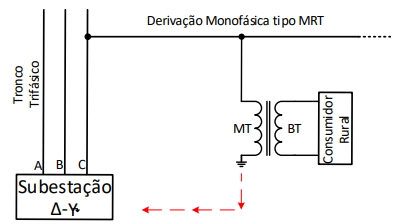
\includegraphics[width=0.8\textwidth]{figuras/Imagem1Fandi2013.png}
	\caption*{Fonte: Adaptado de \cite{fandi_sistema_2013}}
	\label{fig:RedeMonofasicaComRetornoPorTerraAdptadoFandi2013}
\end{figure}

\subsection{Redes Monofásicas com Retorno por Terra (MRT) Não Isoladas ou Neutro Parcial}

\par As redes Monofásicas com Retorno pela Terra (MRT) são sistemas eletricamente não isolados, caracterizados por sua derivação direta de uma única fase de um alimentador trifásico. A funcionalidade do circuito de retorno via solo é dependente da configuração da subestação de origem, a qual deve possuir uma conexão em estrela com neutro solidamente aterrado. Nos transformadores de distribuição instalados ao longo da linha MRT, o enrolamento primário estabelece a conexão entre o condutor de fase e o sistema de aterramento local.

\par Embora esta topologia apresente vantagens significativas devido à sua simplicidade construtiva e operacional, sua aplicação exige uma análise criteriosa do balanceamento de fases na rede trifásica de suprimento. Tal avaliação é fundamental para prevenir a introdução de desequilíbrios de carga excessivos na rede originária. Como medida para assegurar a operação adequada e mitigar potenciais desequilíbrios, a potência instalada em ramais MRT é comumente limitada – um valor referencial frequentemente adotado é de 25 kVA. Adicionalmente, a performance e a segurança da topologia podem ser otimizadas através da implementação de múltiplos pontos de aterramento distribuídos ao longo do circuito conforme visto na Figura \ref{fig:RedeMonofasicaComRetornoPorTerraNeutroParcialAdptadoFandi2013}.

\begin{figure}[H]
	\centering
	\caption{Rede Monofilar com Retorno por Terra (MRT) com Neutro Parcial.}
	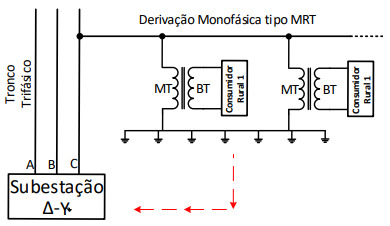
\includegraphics[width=0.8\textwidth]{figuras/Imagem2Fandi2013.png}
	\caption*{Fonte: Adaptado de \cite{fandi_sistema_2013}}
	\label{fig:RedeMonofasicaComRetornoPorTerraNeutroParcialAdptadoFandi2013}
\end{figure}

\subsection{Redes Monofásicas com Retorno por Terra (MRT) com Transformador Isolador}

\par Uma variante das redes Monofásicas com Retorno pela Terra (MRT) emprega um transformador isolador. Diferentemente da derivação direta de uma única fase, esta configuração é alimentada por duas fases da rede trifásica de suprimento. O transformador isolador, frequentemente com relação de espiras de 1:1, tem seu enrolamento primário conectado entre essas duas fases. O enrolamento secundário fornece uma única fase de saída e possui um terminal conectado a um sistema de aterramento local dedicado. Uma vantagem primordial desta topologia é a redução significativa do percurso da corrente de retorno pelo solo, confinando-a essencialmente ao circuito secundário do transformador isolador, o que contribui para a segurança operacional.

\par Adicionalmente, o uso do transformador isolador apresenta benefícios técnicos relevantes. Ele previne a dessensibilização dos dispositivos de proteção de neutro da rede trifásica principal (localizados a montante), garantindo que estes atuem corretamente para faltas fase-terra que ocorram fora do ramal MRT. Outra vantagem reside na possibilidade de um melhor controle de tensão no circuito monofásico, incluindo o ajuste fino através dos taps do próprio transformador isolador.

\par Entretanto, a implementação desta configuração acarreta desvantagens. Primeiramente, há um custo adicional associado tanto ao transformador isolador quanto ao seu sistema de aterramento específico. Do ponto de vista da proteção elétrica, o trecho MRT após o isolador torna-se uma "zona cega" (fora do alcance) para relés sensíveis a faltas para terra situados a montante do transformador. Consequentemente, a proteção para faltas internas nesse trecho depende primariamente de dispositivos de sobrecorrente de fase, também localizados a montante. Por fim, a complexidade do sistema é incrementada, especialmente no que concerne ao projeto e execução do aterramento do transformador isolador, o qual, dependendo de suas características, pode impor limitações à potência máxima transferível ao ramal monofásico.

\subsection{Para Raio Energizado (PRE)}

\par O sistema Monofásico com Retorno pela Terra (MRT), concebido por Mandeno ()\citeyear{mandeno_rural_1947}), não apenas solucionou desafios da época, mas também estimulou a pesquisa em novas tecnologias para transmissão e distribuição de energia elétrica. Inspirados por essa premissa, Iliceto et al. (\citeyear{iliceto_new_1989}) desenvolveram um sistema inovador denominado Para-Raios Energizado (PRE). A concepção original baseou-se na isolação e energização dos cabos para-raios (originalmente destinados apenas à proteção contra descargas atmosféricas) de uma linha de transmissão de 161 kV em Gana. O sistema PRE demonstrou flexibilidade, podendo operar em quatro configurações distintas.

\par As configurações descritas por Iliceto et al. (\citeyear{iliceto_new_1989}) são:
\begin{itemize}
	\item \textbf{Monofásica com Retorno pelo Solo}: Apenas um cabo para-raios é energizado, utilizando o solo como caminho de retorno, similar ao MRT.
	\item \textbf{Monofásica com Retorno Metálico}: Ambos os cabos para-raios são energizados, um servindo como condutor de fase e o outro como retorno.
	\item \textbf{Trifásica em Delta Aberto}: Ambos os cabos são energizados, alimentando transformadores em conexão V (delta aberto) para cargas trifásicas, porém com limitações (tipicamente restrito a cargas fase-neutro).
	\item \textbf{Trifásica com Retorno pelo Solo}: Os dois cabos para-raios atuam como duas fases, e o solo é utilizado como terceiro condutor de fase. Esta configuração, apesar de apresentar complexidades relacionadas à impedância do solo e acoplamentos capacitivos entre condutores e solo, é considerada a mais adequada para o suprimento de cargas trifásicas.
\end{itemize}

\par O sistema PRE de Iliceto et al. (\citeyear{iliceto_new_1989}), derivado conceitualmente do MRT de Mandeno (\citeyear{mandeno_rural_1947}), representa um avanço tecnológico significativo para atender à crescente demanda energética em áreas rurais próximas a linhas de transmissão existentes.

\par No Brasil, a quarta configuração do PRE (trifásica com retorno pelo solo) foi implementada no estado de Rondônia, através de um projeto colaborativo entre a Eletronorte e as Centrais Elétricas de Rondônia (Ceron). A análise dos dados operacionais deste sistema, realizada por Rose (\citeyear{rose_alimentacao_1997}), demonstrou sua viabilidade técnica e econômica como alternativa para a universalização do acesso à energia. O estudo concluiu que o PRE possibilita o fornecimento a pequenas comunidades ou cargas isoladas adjacentes às linhas de transmissão, onde a extensão de redes convencionais seria economicamente proibitiva.

\par Os resultados encorajadores do PRE Rondônia estimularam pesquisas complementares. Ramos (\citeyear{ramos_universalizacao_2010}) conduziu um estudo detalhado sobre as interrupções do sistema, avaliando seu desempenho frente a descargas atmosféricas e estabelecendo índices operacionais específicos. Além disso, analisou o fenômeno da tensão induzida por acoplamento capacitivo e documentou a implementação de um regulador de tensão baseado em sintonização de ressonância para mitigar esse efeito. Em conjunto, os estudos de Rose (\citeyear{rose_alimentacao_1997}) e Ramos (\citeyear{ramos_universalizacao_2010}) indicam que a tecnologia PRE, quando implementada segundo seus conceitos fundamentais, atende aos requisitos essenciais de qualidade e segurança para o fornecimento de energia elétrica.

\pagebreak

\subsection{Sistema Trifásico a Dois Fios (T2F)}

\par O sistema Monofásico com Retorno pela Terra (MRT) fundamenta-se na utilização de um único condutor aéreo para a fase, enquanto o retorno da corrente se efetua através de sistemas de aterramento localizados em cada ponto de transformação (transformador de distribuição). Esta configuração intrinsecamente simplifica a construção da rede, tornando-a mais rápida e economicamente vantajosa (Kräulich et al., 2023). As principais vantagens derivam dessa simplicidade: estações transformadoras menos complexas e de menor custo, transformadores com apenas uma bucha de alta tensão, e, consequentemente, a exigência de somente um para-raios e uma chave fusível monofásica por unidade transformadora.

\par Contudo, o cenário de aumento de carga nas propriedades rurais frequentemente impõe a necessidade de migração de sistemas monofásicos para trifásicos. A conversão de uma rede MRT existente para uma trifásica convencional representa um desafio considerável para as concessionárias. O custo elevado da construção de uma nova infraestrutura trifásica é um fator primordial, especialmente porque nem sempre é estruturalmente viável simplesmente adicionar dois condutores aéreos à estrutura de postes originalmente projetada para o sistema MRT.

\par Nesse contexto, o sistema Trifásico a Dois Fios (T2F) apresenta-se como uma alternativa tecnológica para a repotencialização de redes MRT. Uma característica chave do T2F é o aproveitamento da infraestrutura existente: ele utiliza um dos aterramentos já presentes na rede MRT e permite, em muitos casos, a manutenção da estrutura de postes. A adaptação envolve a instalação de um transformador isolador trifásico específico, que possui uma das fases secundárias aterrada e as outras duas conectadas aos condutores aéreos (o original e um adicional). Com isso, a estrutura básica do SWER/MRT pode ser mantida, necessitando apenas de um isolador e uma chave fusível adicionais em relação ao sistema monofásico original.

\par A implementação e operação do sistema T2F, esquematizado na Figura \ref{fig:RedeT2FAdptadoMarchesan2023}, demandam atenção a aspectos de segurança relacionados à injeção de corrente no solo, inerente ao seu princípio de funcionamento com retorno parcial ou total pela terra. É fundamental realizar análises de segurança contra choque elétrico, seguindo padrões internacionais como a norma IEEE Std 80. Esta norma estabelece metodologias para avaliar os gradientes de potencial gerados pelo fluxo de corrente no solo nas proximidades dos eletrodos de aterramento. O guia da IEEE aborda conceitos essenciais para essa avaliação, como a corrente máxima tolerável pelo corpo humano, cenários de aterramento acidental e os critérios para determinação das tensões de segurança toleráveis (tensões de toque e passo).

\begin{figure}[H]
	\centering
	\caption{Rede proposta por Marchesan.}
	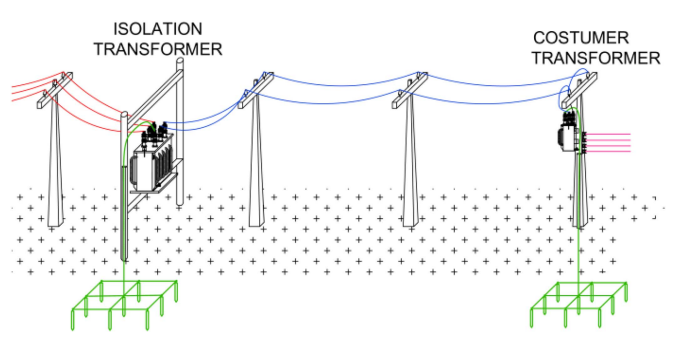
\includegraphics[width=0.8\textwidth]{figuras/Imagem3T2F2023.png}
	\caption*{Fonte: Adaptado de \cite{marchesan_three-phase-two-wire_2023}}
	\label{fig:RedeT2FAdptadoMarchesan2023}
\end{figure}

\par Embora o sistema Trifásico a Dois Fios (T2F) possua similaridades com outras tecnologias como o PRE, ele apresenta características particulares que são cruciais para sua correta implementação e operação, conforme destacado por Marchesan et al. (\citeyear{marchesan_three-phase-two-wire_2023}) pela Figura \ref{fig:RedeT2FAdptadoMarchesan2023}. Destacam-se os seguintes pontos:

\begin{itemize}
	\item \textbf{Transformador de Isolação Mandatório}: A implementação do T2F requer obrigatoriamente um transformador de isolação específico. Este atua como interface entre a rede de suprimento trifásica convencional e a linha T2F não convencional.
	\item \textbf{Configuração do Transformador}: O primário deste transformador é alimentado por tensão trifásica simétrica. No secundário, uma das três fases é solidamente aterrada no local, enquanto as outras duas fases são conectadas aos condutores aéreos da linha T2F.
	\item \textbf{Capacidade de Suprimento Trifásico}: O sistema T2F é capaz de suprir cargas trifásicas balanceadas (até 100\% da capacidade) utilizando transformadores de distribuição Média Tensão/Baixa Tensão (MT/BT) convencionais, desde que estes possuam conexão primária em delta (ou outra que não exija neutro) e secundária em estrela-aterrada. Isso permite, por exemplo, a alimentação de motores de indução trifásicos de maior porte, essenciais para diversas atividades rurais.
	\item \textbf{Segurança do Aterramento}: A circulação de corrente pelo solo, inerente à topologia, exige um projeto criterioso do sistema de aterramento. É imperativo garantir a segurança de seres humanos e animais (controle de tensões de toque e passo), prevenir aquecimento excessivo do solo e evitar interferência eletromagnética em sistemas de comunicação adjacentes.
\end{itemize} 

\par O objetivo primário da instalação do transformador isolador é isolar galvanicamente o circuito T2F da rede de alimentação principal. Essa isolação restringe a propagação de correntes de falta (especialmente as de sequência zero) para a rede a montante, o que facilita o controle das tensões de passo e de toque no trecho T2F durante condições anormais. Dada a criticidade do sistema de aterramento, recomenda-se o monitoramento periódico da sua integridade, tanto no ponto do transformador isolador quanto nos pontos de aterramento dos transformadores dos consumidores.

\par Finalmente, as condições de alimentação no primário do transformador isolador T2F são compatíveis com os níveis de tensão de média tensão (MT) padronizados e usualmente empregados pelas concessionárias para alimentar redes trifásicas convencionais em zonas rurais.



% % % % % % % % % % % % % % % % % % % % % % % % % % % % % % % % % % % % % % 
% % % % % % % % % % % % FIM DAS PAGINAS TEXTUAIS % % % % % % % % % % % % % % 
% % % % % % % % % % % % % % % % % % % % % % % % % % % % % % % % % % % % % % 
% % % % % % % % % % % % % % % % % % % % % % % % % % % % % % % % % % % % % % 	
% % % % % % % % % % % % % BIBLIOGRAFIA  % % % % % % % % % % % % % % % % % % 
% % % % % % % % % % % % % % % % % % % % % % % % % % % % % % % % % % % % % % 	

\startbibliography % comando para formatar na MDT UFSM
\bibliography{ArtigosTese} %%% NOME DO ARQUIVO .bib
% % % % % % % % % % % % % % % % % % % % % % % % % % % % % % % % % % % % % 	
% % % % % % % % % % % % % APENDICES % % % % % % % % % % % % % % % % % % %
% % % % % % % % % % % % % % % % % % % % % % % % % % % % % % % % % % % % % 	
%% \apendice %%%% TEXTOS A PARIR DESTE PONTO SERAO CONSIDERADOS APENDICES

% % % % % % % % % % % % % % % % % % % % % % % % % % % % % % % % % % % % % % 	
% % % % % % % % % % % % % % % ANEXOS  % % % % % % % % % % % % % % % % % % % 
% % % % % % % % % % % % % % % % % % % % % % % % % % % % % % % % % % % % % % 	
%% \anexo    %%%% TEXTOS A PARIR DESTE PONTO SERAO CONSIDERADOS ANEXOS     
\end{document}